\documentclass[11pt,a4paper]{article}
\usepackage[margin=2.5cm]{geometry}
\usepackage[T1]{fontenc}
\usepackage{lmodern}
\usepackage{microtype}
\usepackage{amsmath,amssymb,bm}
\usepackage{graphicx}
\usepackage{xcolor}
\usepackage{caption}
\captionsetup{font=small,labelfont=bf}
\usepackage[breaklinks=true]{hyperref}
\hypersetup{colorlinks=true,linkcolor=blue!60!black,urlcolor=blue!55!black,
  citecolor=blue!60!black}

\title{\textbf{The phase-winding bit: how much noise does a topological
invariant actually survive?}\\[3pt]
\large A quantitative note, with a correction of one common misapplication}
\author{O.~Kirichenko\\[2pt]\small
  \href{mailto:urevich55@gmail.com}{urevich55@gmail.com}}
\date{\today}

\begin{document}
\maketitle

\begin{abstract}\noindent
``Information stored in a topological invariant is protected against
continuous deformation'' is a true and powerful statement---it underlies
topological quantum error correction and won recognition in the 2016
Nobel Prize for topological phases of matter. It is also frequently
\emph{misapplied}, e.g. to claim that a macroscopic object could be
``dissolved and reconstructed'' because its structure is topologically
encoded. This note does two things. First, it makes the true statement
\emph{quantitative} for the simplest topological memory---the winding
number of a phase field---by Monte-Carlo: the winding survives local
Gaussian phase noise up to a sharp threshold ($\sigma\!\approx\!0.6$~rad
here), below which the bit-error rate falls exponentially as
$\sim\!N\,\mathrm{erfc}(\pi/2\sigma)$ (Fig.~\ref{fig:bit}). Second, it
draws the honest boundary: the same integer winding that robustly stores
\emph{one bit} (and that appears, correctly, as the topological charge in
the arrow-of-time argument of the NVG framework) cannot store the
$\sim\!10^{26}$ independent coordinates of a macroscopic body---the
protection is real, but its information capacity is $\log_2$ of the number
of topological sectors, not the phase-space volume.
\end{abstract}

\section{The claim, and where it goes wrong}
A phase field $\theta(x)\in[0,2\pi)$ on a ring carries a winding number
\begin{equation}
  W = \frac{1}{2\pi}\oint \partial_x\theta\,dx
    = \frac{1}{2\pi}\sum_i \mathrm{wrap}(\theta_{i+1}-\theta_i)
    \in\mathbb{Z},
\end{equation}
where $\mathrm{wrap}$ maps a difference into $(-\pi,\pi]$. $W$ is an
\emph{integer}: no continuous, local deformation of $\theta$ can change it,
because to do so some link difference must cross $\pm\pi$---a discrete
``phase slip''---which a smooth deformation never forces. This is the
prototype of topological protection: the stored datum ($W$) is a global
property, invisible to and unchangeable by local perturbations, until they
are large enough to tear the field.

The correct uses of this fact are among the deepest in modern physics:
Kitaev's toric code and the surface codes store logical qubits in the
homology (winding) sectors of a lattice, protected against local errors up
to a threshold~\cite{kitaev,dennis}; the 2016 Nobel Prize recognised
topological order and the role of winding invariants in matter~\cite{nobel}.
Within the NVG/VMF framework the \emph{same} integer appears legitimately
as the topological charge $Q=\tfrac{1}{2\pi}\oint d\theta=1$ that fixes the
sign of entropy production in the arrow-of-time argument.

The \emph{mis}application is to read ``topologically protected'' as
``arbitrarily much information, indestructibly stored.'' A winding number
protects exactly $\log_2(\text{number of accessible sectors})$ bits---one
bit per independent $\mathbb{Z}$ (or $\log_2 d$ for a $d$-sector code), not
the $\sim\!10^{26}$ real numbers specifying the atomic coordinates of a
kilogram of matter. Topology protects the \emph{label}, not the
\emph{library}.

\section{How much noise does one winding bit survive?}
We store $W=1$ as the smooth state $\theta_i=2\pi i/N$ on a ring of
$N=64$ sites, add independent Gaussian noise
$\theta_i\to\theta_i+\mathcal{N}(0,\sigma)$, and measure the probability
that the winding is still $1$. Figure~\ref{fig:bit}a shows a sharp
survival transition; Fig.~\ref{fig:bit}b shows the bit-error rate.

\begin{figure}[t]
\centering
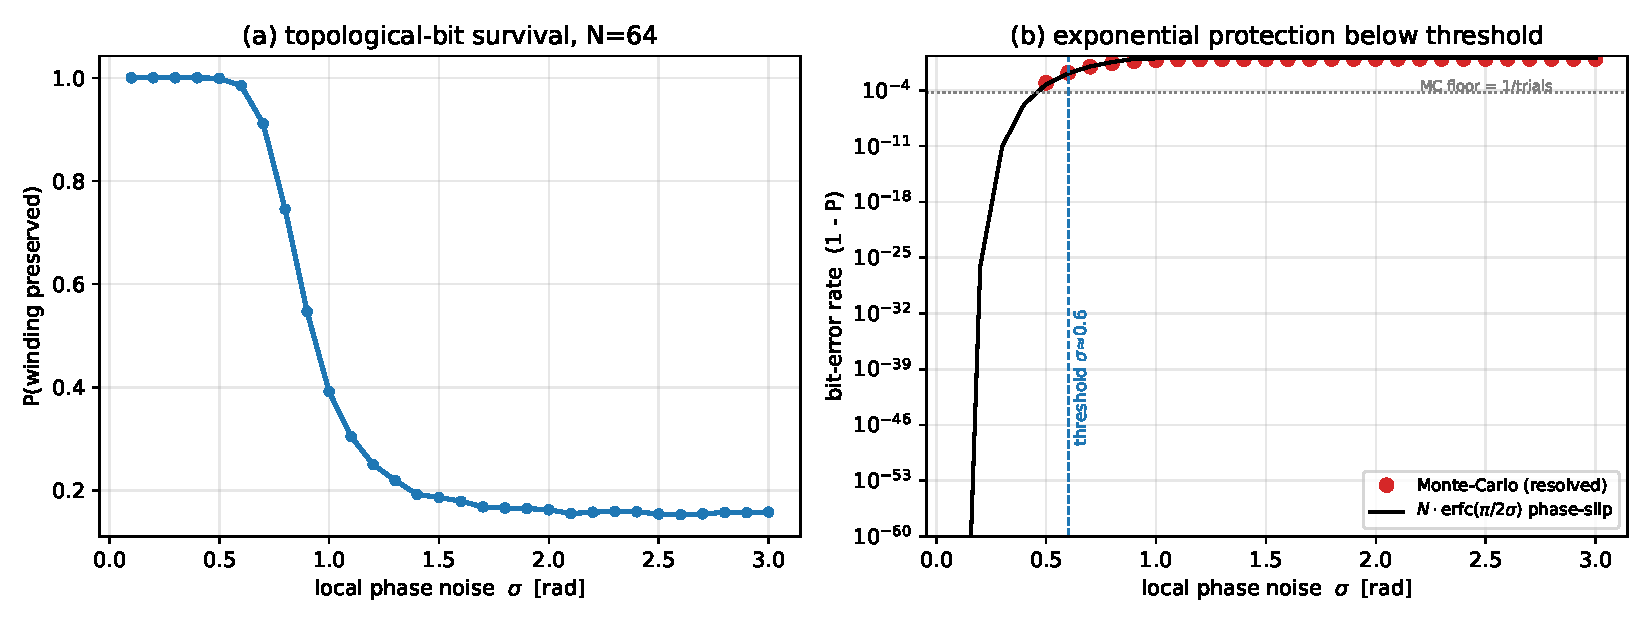
\includegraphics[width=\textwidth]{fig_winding_bit.pdf}
\caption{\textbf{(a)} Probability that the winding number is preserved vs
local phase-noise amplitude $\sigma$ ($N=64$, $2\times10^4$ Monte-Carlo
trials). The bit is essentially perfectly protected below
$\sigma\!\approx\!0.6$~rad and randomises above $\sigma\!\sim\!1$~rad.
\textbf{(b)} Bit-error rate: Monte-Carlo (points, resolution-limited to
$1/\text{trials}$) against the analytic phase-slip estimate
$N\,\mathrm{erfc}(\pi/2\sigma)$ (line), which falls exponentially below
threshold---the signature of topological protection. Reproduced by
\texttt{winding\_bit.py}.}
\label{fig:bit}
\end{figure}

Two quantitative lessons:
\begin{itemize}
\item \textbf{A threshold, not a wall.} Below $\sigma_c\!\approx\!0.6$~rad
  the error is exponentially small---$N\,\mathrm{erfc}(\pi/2\sigma)$, e.g.
  $\sim\!10^{-23}$ at $\sigma=0.3$ for $N=64$---so the bit is stable for
  cosmological times. Above threshold it randomises. Protection is
  parametric, controlled by the ratio (noise)/(tear scale $\pi$), exactly
  as topological quantum codes have an error threshold.
\item \textbf{Capacity scales, robustness dilutes.} The error grows
  linearly with system size at fixed $\sigma$ ($0.34,0.60,0.82$ for
  $N=16,64,256$): more links means more chances for a phase slip. A larger
  medium stores \emph{more} winding sectors (more bits) but each individual
  bit is \emph{easier} to break---the standard capacity/robustness trade
  that real topological codes resolve with redundancy and active
  correction.
\end{itemize}

\section{The honest boundary}
The winding bit is the correct, minimal realisation of the intuition
``structure encoded in a topological invariant resists continuous
deformation.'' Its value---and its limit---are now numbers:
\begin{enumerate}
\item it stores $\log_2(\#\text{sectors})$ bits, robustly, with an
  explicit noise threshold;
\item it does \emph{not} store a macroscopic configuration: topology
  protects a discrete label whose capacity is logarithmic in the number of
  sectors, astronomically short of the phase-space of a solid body;
\item the same invariant is used correctly elsewhere---toric/surface codes
  for qubits, and the topological charge $Q=1$ in the NVG arrow-of-time
  argument---while the ``teleport a body by topological encoding'' reading
  fails on the capacity count alone, before any dynamical objection.
\end{enumerate}
The general moral is a useful filter: whenever ``topologically protected''
is invoked, ask \emph{how many bits} the invariant actually carries and
\emph{what tears it}. Both are computable, as above; a claim that survives
both is real physics, and one that needs the invariant to carry
macroscopic information is not.

\section*{Code and data}
\texttt{winding\_bit.py} reproduces the figure, the threshold and the
$N$-scaling (ring phase field, exact integer winding, Monte-Carlo over
local Gaussian noise).

\begin{thebibliography}{9}\small
\bibitem{kitaev} A.~Yu.~Kitaev, ``Fault-tolerant quantum computation by
  anyons,'' Ann.\ Phys.\ \textbf{303} (2003) 2 [quant-ph/9707021].
\bibitem{dennis} E.~Dennis, A.~Kitaev, A.~Landahl, J.~Preskill,
  ``Topological quantum memory,'' J.\ Math.\ Phys.\ \textbf{43} (2002)
  4452.
\bibitem{nobel} The Nobel Prize in Physics 2016 (D.~J.~Thouless,
  F.~D.~M.~Haldane, J.~M.~Kosterlitz), ``for theoretical discoveries of
  topological phase transitions and topological phases of matter.''
\end{thebibliography}

\end{document}
